\chapter{Etude terrain} % 30 pages

	\paragraph{Comment j'ai réalisé mon étude terrain ? \\}

		Lors de mon étude terrain, j'ai eu l'occasion de recenser l'avis de nombreuses personnes sur l'open source mais également sur les réflexions menée lors de mon état de l'art.
		J'ai choisi d'orienter mes questions autour des 4 grands domaines qui représentent selon moi les piliers à batir pour valoriser l'open source, et sur lesquel l'éditeur à la main.

		\subparagraph{Etude quantitative \\}

		Pour cette étude terrain j'ai pu réaliser un sondage de 13 questions autour de ma problématique qui à pu être traité par 39 personnes qui sont lié de près ou de loin à l'open source. Cette étude quantitative me permet de vérifier la véracité de mes hypothèses en cherchant le maximum d'approbation mais aussi de désapprobation de mes idées et réflexions.

		\subparagraph{Etude qualitative \\}

		L'étude qualitative que j'ai pu réalisé au travers de 4 interviews, m'a permis de confronter mes idées à celles d'autre personnes sensibles au domaine de l'open source . Ceci m'aide à étayer mes réflexions à travers leurs visions.

	\section{Plateforme promotrice}

		\subsection{Une interface pour communiquer qui laisse à désirer}

			Autour des plateformes qui contiennent et promouvoie l'open source, sur 39 réponses enregistrées pour cette question, 20 indiquent qu'il y a un manque à palier dans l'interface qui permet de communiquer avec l'éditeur open source. 

			\begin{figure}[!htb]
				\center
				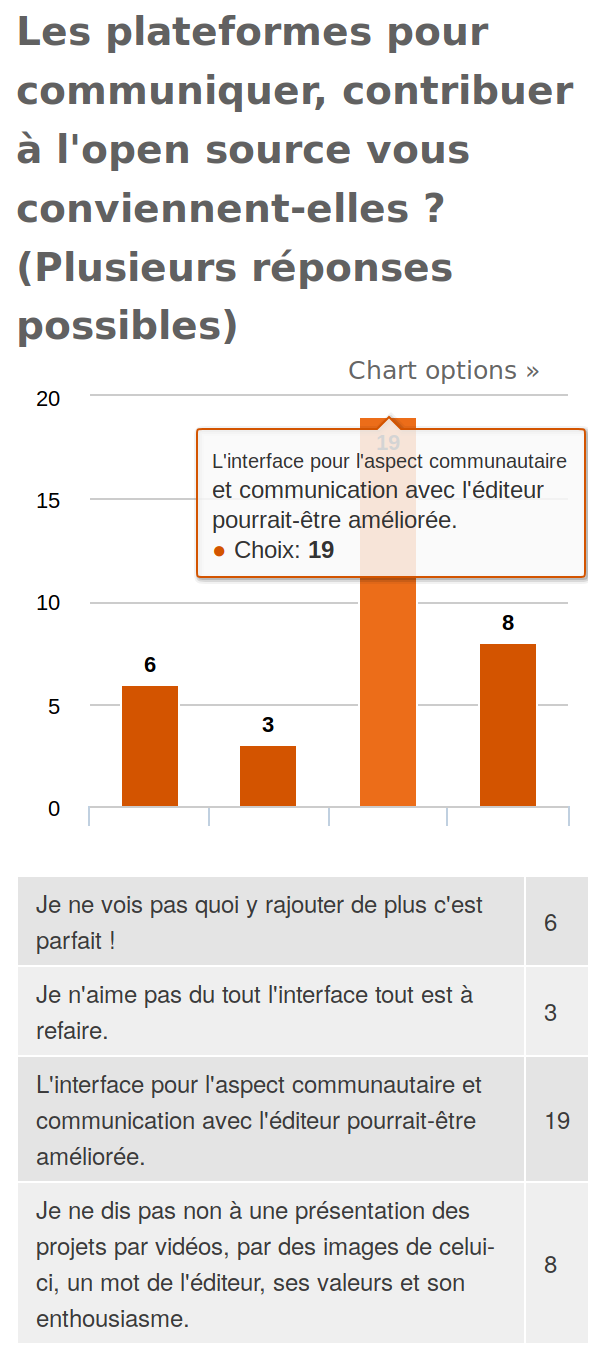
\includegraphics[scale=0.28]{./img/a9}
				\caption{Communication avec l'éditeur}
			\end{figure}

			Il apparait donc que \textbf{la communication qui a un aspect fondamental} pour l'open source \textbf{peux clairement être améliorée} afin de satisfaire non seulement les besoins dans la communication auprès de l'éditeur mais surtout le besoin du consommateur à communiquer correctement.\\

			Lors de l'interview auprès de Olivier \bsc{Magnial}, ingénieur systèmes embarqués chez l'une des plus grande entreprise promotrice de l'open source : SMILE. Celui-ci à déclaré : 

			\begin{center}
				\textit{
				\textquote{
					Pour \gls{mainliner} du code source, un processus décrit la manière de contribuer, et c'est le plus souvent par mail.(...) Linux, par exemple c'est entièrement du mail, on à des mailing list extrêmement longues et des processus assez carrés !
				}
				}
			\end{center}

			Florent Garin, CEO de Docdoku et éditeur du logiciel open source DocdokuPLM, s'exprime sur le sujet en rapportant qu'il y a un problème sur ces plateformes pour communiquer avec les contributeurs:

			\begin{center}
				\textit{
				\textquote{
					On passe beaucoup de temps à éduquer les potentiels contributeurs car ils confondent contribution en relevant des anomalies et demandes de support (...) Un système de tag plus explicites sur les \gls{issues} améliorerait cette communication.
				}
				}
			\end{center}

			Finalement pour Florent Garin, un axe d'amélioration de l'éditeur auprès du contributeur serait la mise en place de guide, de documentation sur comment contribuer et d'un ticket spécial "first contribution".\\

			Ainsi, \textbf{ce n'est pas au travers des plateformes que cette communication pour la contribution est la plus utile et pratique et des moyens peuvent être mis en oeuvre pour améliorer la communication}.\\

			De plus la prise en main d'un logiciel open source est souvent plus compliqué nous révèle Quentin \bsc{Cazelle}, ingénieur logiciel chez Docdoku.\\

			Pourquoi selon lui ?

			\begin{center}
				\textit{
				\textquote{
					Car il y a des fonctionnalités non documentées (...) les plateformes sont incomplètes car les développeurs qui contribuent au projets open source ne s'embêtent pas à la documentation et a bien expliquer les issues.
				}
				}
			\end{center}

			J'en déduis donc qu'en plus d'une communication pouvant être amélioré, \textbf{faciliter l'écrit autour des contributions et sensibiliser les consommateurs à la documentation} est un axe d'amélioration potentiel.

		\subsection{Un module de présentation}

			Sur la question:

			\begin{center}
				\textit{
				\textquote{
					Les plateformes pour communiquer, contribuer à l'open source vous conviennent-elles ?
				}
				}
			\end{center}

			Seulement 8 personnes sont intéressés pour avoir une présentation sous forme de vidéo du projet, avec un mot de l'éditeur qui communique ses ambitions, ses valeurs.

			\begin{figure}[!htb]
				\center
				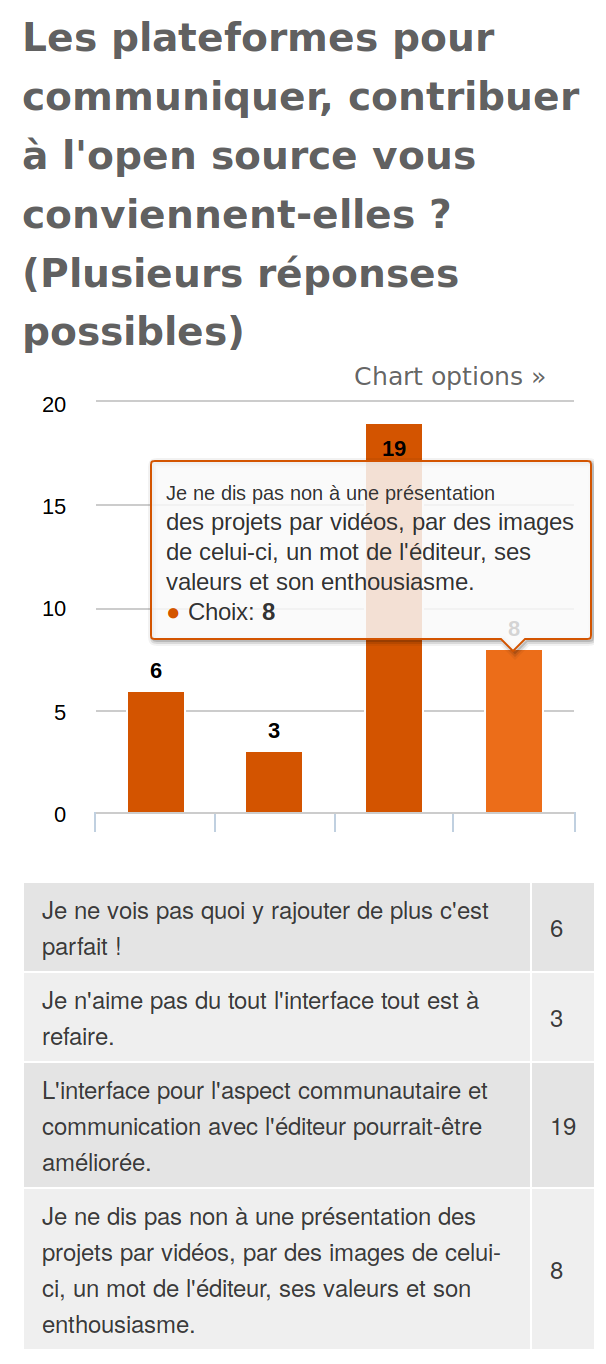
\includegraphics[scale=0.28]{./img/a92}
				\caption{Module de présentation}
			\end{figure}

			Lors de l'interview de Quentin \bsc{Cazelle}, Ingénieur développeur chez Docdoku, celui-ci mentionne tout de même le fait qu'une vitrine à ces plateformes s'impose pour les consommateurs finaux qui ne sont pas développeur.

			\begin{center}
				\textit{
				\textquote{
					La plateforme est un frein pour l'utilisateur final non développeur, il faudrait en effet mettre une vitrine dans un style plus commercial (...)
				}
				}
			\end{center}

			Florent \bsc{Garin}, mentionne quant à lui que le support de présentation par vidéo ne se prête pas à ce sujet.

			\begin{center}
				\textit{
				\textquote{
					La vidéo c'est souvent pour présenter des produits grands public, je pense pas que ce soit un bon moyen de communiquer sur l'open source car l'open source c'est majoritairement des projet ou des "briques" logicielles techniques.
				}
				}
			\end{center}

			J'en conclus qu'\textbf{une présentation du logiciel n'est pas pertinente} pour le développeur contributeur ou les entreprises consommatrices.

		\subsection{Pas d'extrèmes sur les plateformes}

			Très peu de contributeur, c'est-à-dire 8 sur 30, répondent que les plateformes sont parfaites et qu'ils ne voient pas d'amélioration potentielles.\\

			Il n'y a pas non plus beaucoup d'insatisfait sur celles-ci car seulement 3 ont répondu que toute l'interface était à refaire.\\

			Je trouve donc que \textbf{les plateformes promotrices sont utilisés et essentielles} à l'open source et dont l'éditeur ne dois pas faire l'impasse.

	\section{Gestion des ressources}

		\subsection{Un mot de l'éditeur pour valoriser la contribution}

			Florent \bsc{Garin} mentionne qu'un projet open source est décentralisé et que malgré le leader potentiel (l'éditeur) qui approuve les contributions, l'open source n'est pas hierarchisé et donc ne se résume pas aux valeurs et missions de l'éditeur.

			\begin{center}
				\textit{
				\textquote{
					 (...), il y a un leader qui possède le repertoire avec le code mais ce n'est pas si hiérarchisé que celà, l'open source doit être vu comme un pot commun dans lequel tout le monde pioche.
					 Même si l'éditeur ou l'entreprise peut avoir un avantage financier, le projet est assez décorélé d'elle, le code que je met m'appartient quasiemment autant qu'a l'entreprise derrière (en fonction des licences), chacun doit chercher à contribuer dans le pot commun car ils se servent du logiciel et non pour la mission derrière ou les valeurs incarnées de l'éditeur.
				}
				}
			\end{center}

			Lors de l'interview de Quentin \bsc{Cazelle}, il souligne cette séparation de l'éditeur et de la communauté.
			\begin{center}
				\textit{
				\textquote{
					 Ce n'est pas une entreprise qui à un besoin, c'est une communauté avec des besoins !
				}
				}
			\end{center}


			Il n'y a donc finalement pas vraiment d'échange avec les valeurs et missions de l'initiateur du projet open source \textbf{mais plus une communication autour du besoin qu'a le consommateur et la communauté et donc les potentiels contributeurs à créer ce projet open source}

		\subsection{Pas de niveau hiérarchique}

			Lors de mon interview avec Quentin \bsc{Cazelle}, il m'informe que les relations hiérarchiques dans l'open source sont plutot implicites.

			\begin{center}
				\textit{
				\textquote{
	 				Si j'arrive sur un projet open source et que les gens connaissent bien le projet, il sont "au dessus" de moi, si moi je monte en compétence alors ma voix vaudra la leur. (...) Ce sont des rapports qui se construisent implicitement, cela se joue au mérite. (...) L'éditeur au final c'est juste lui qui à le dernier mot pour intégrer la contribution.
				}
				}
			\end{center}

			Ce qui rejoint le point de vue de Florent \bsc{Garin}, qui m'informe que la relation hiérarchique dans un projet open source est inexistante, l'éditeur ne peux pas contrôler les contributeur, ni assigner de tâche (que je précise ultérieurement).\\

			J'en conclus que\textbf{cet aspect hiérarchique de l'open source n'est qu'illusion et que seul réside la communication} entre les individus contributeurs et les acceptations de contribution par l'éditeur.

		\subsection{La gestion des projets open source}

			Une question a été traité autour de la gestion de projet open source et la méthode de gestion.
			J'ai donc sollicité l'imagination des personnes interrogé en leur demandant de se mettre à la place de l'éditeur open source.\\

			Ainsi en tant qu'éditeur, qu'aimeraient-ils de leur communauté concernant la participation ?\\

			28 personnes sur 39 ont ainsi répondu qu'ils aimeraient se mettre au meme niveau que la communauté et qu'en tant qu'éditeur ils contribuent de la même façon que la communauté.\\

			Seulement 10 ont répondu qu'ils aimerait se charger du noyau et que le développement de module et d'extensions à intégrer est attribué à la communauté.\\

			1 seule personne à répondu qu'elle n'aimaient pas l'aspect communautaire de l'open source.

			\begin{figure}[!htb]
				\center
				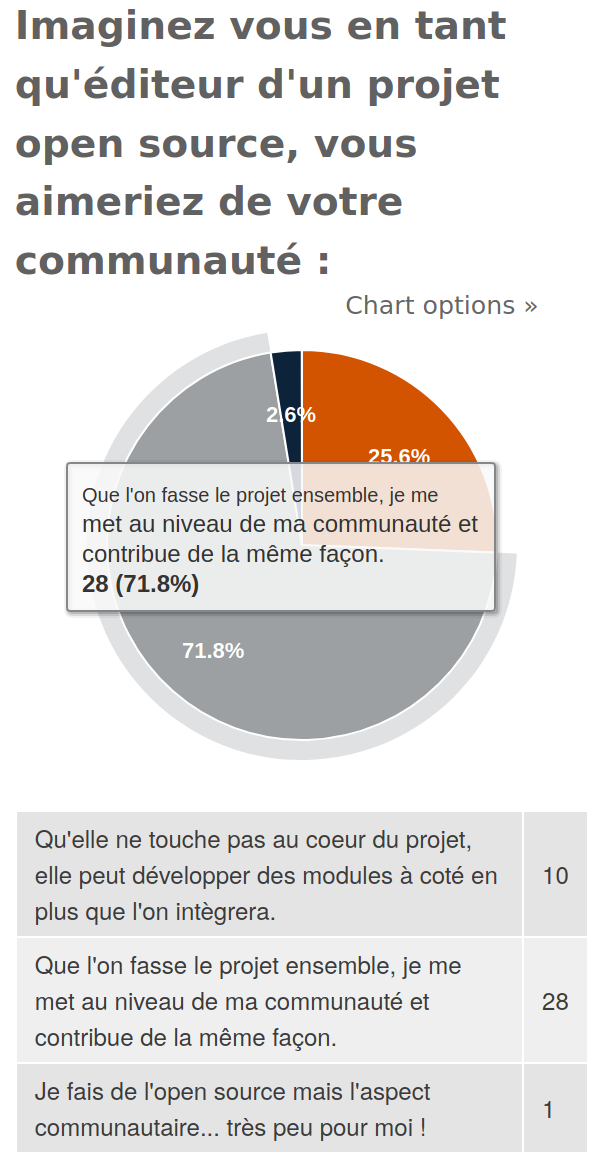
\includegraphics[scale=0.28]{./img/communaute}
				\caption{Gestion de communauté en tant qu'éditeur}
			\end{figure}

			Quentin \bsc{Cazelle} lui exprime que les besoins dans le modèle de noyau/extension sont tous différents pour chaque contributeur ou consommateur et cela pose un problème de simplicité du logiciel résultant qu'il est difficile de gérer.

			\begin{center}
				\textit{
				\textquote{
					 Il peux y avoir des besoins contradictoires, qui ramènent beaucoup de complexité, dans mon ancienne société, notre besoin était simple et le logiciel est 4 fois trop gros, il est difficile de séparer le noyau des extensions car l'intégrité du code n'est pas garantie, les mises à jours peuvent être compliqués.
				}
				}
			\end{center}

			De plus il souligne que le développement d'extension pour un besoin spécifique devient intéressant à faire payer alors qu'une modification du coeur du projet doit être partagée à l'ensemble de la communauté.\\

			J'en déduis qu'un mode de gestion noyau/extension n'est pas forcément bien perçu ou logique pour les personnes interrogés et que l'aspect de communauté et de management horizontal est mieux à leurs yeux. Ainsi \textbf{travailler de pair avec l'éditeur sans impression de dénivelé de pouvoir est préférable}.\\

			Florent Garin mentionne quand à lui qu'il y a plusieurs business model autour de l'open source mais qu'il y a très peu de succès.

			\begin{center}
				\textit{
				\textquote{
					 Dans les business model présent, il y a celui ou les développeurs se réunissent autour d'un besoin commun et réalisent un projet open source à but non lucratif et c'est souvent ce qui marche le mieux finalement, comme le noyau linux, personne ne gagne de l'argent directement avec le noyau linux, et c'est la mutualisation d'un effort commun qui prime.
				}
				}
			\end{center}

			Egalement, selon lui, ce modèle noyau/extension ne prévaut pas, il faut faire attention aux entreprises "prédatrice" et qui mettent à mal ces projets.

			\begin{center}
				\textit{
				\textquote{
					 Des exemples, il y en a plein, je pense à Docker qui a crée son projet open source a essayé de développer ses extensions et qui finalement n'a pas vraiment réussi à monétiser cela face à d'autre entreprise avec d'autre aspirations comme Google qui à bien profité de Docker. (...) Ce qui menace le plus l'open source c'est l'hébergement cloud.
				}
				}
			\end{center}

			Aucun modèle n'est mieux qu'un autre souligne Quentin \bsc{Cazelle}, les besoins de l'éditeur varient et il jongle parfois entre autoriser les contribution au coeur de son projet ou accepter les extensions proposées.\\

			Ainsi, je peux en déduire qu'il y a beaucoup de menaces et contraintes autour des projets open source et \textbf{les business models à employer ne résumer à un type en particulier qui va fonctionner généralement}.

		\subsection{La gestion des contributions}

			Afin de gérer les ressources mise à disposition et donc essentiellement la communauté, j'ai posé la question sur comment, en tant que membre de communauté open source, la personne aimerait travailler. A celle-ci, 80\% des personnes ont répondu qu'elles préfèrent toucher un peu à tout dans le projet et gagner en connaissance en sollicitant une multitude de personnes.\\

			Seulement 20\% des personnes souhaiterai monter en compétence dans un seul domaine et y être attribué pour plus de ciblage sur une compétence clé.

			\begin{figure}[!htb]
				\center
				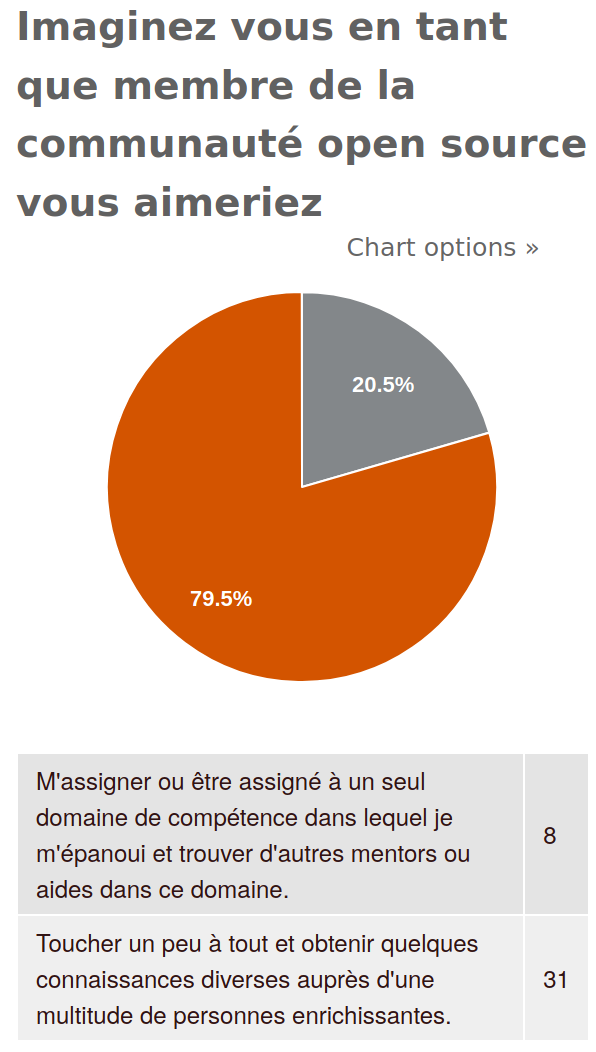
\includegraphics[scale=0.28]{./img/multicompetence}
				\caption{Multi-compétence ou expertise ?}
			\end{figure}

			Pour Quentin \bsc{Cazelle}, le fait de toucher à tout lui est préférable:

			\begin{center}
				\textit{
				\textquote{
					 Cela donne une meilleure compréhension globale du produit, sur le projet open source auquel j'ai participé, j'ai touché à tout et celà m'a permis de pouvoir expliquer le fonctionnement de tout le logiciel en entier.
				}
				}
			\end{center}

			La vision du contributeur est donc de gagner un peu en compétence dans tout les domaines afin d'être polyvalent plutot qu'expert dans un domine précis.\\

			Florent Garin souligne un fait important lors de cette question autour de la gestion des ressources.
			L'open source c'est selon le bon vouloir du contributeur, il n'y a pas de relation hiérarchique, ni de tâche à donner aux contributeurs de ce fait on ne peux pas assigner les contributeurs à un domaine spécifique plutot qu'à un autre.Ainsi tout dépend de la volonté du contributeur.

			\begin{center}
				\textit{
				\textquote{
					 Chacun est libre de faire ce qu'il veut, par contre en tant qu'éditeur, tu es libre d'accepter sa contribution,(...) néanmoins celui qui va contribuer sur un domaine qu'il ne maitrise pas se verra peut être refuser plusieurs fois des contributions.
				}
				}
			\end{center}

			Ainsi \textbf{cela change ma vision sur l'optimisation de ressource humaine et des contribution que je perçevais comme "assignable"} mais qui restent effectivement au bon vouloir du contributeur.

	\section{Chez le consommateur}

		\subsection{La contribution du consommateur}

			Dans les personnes interrogés, beaucoup souhaite contribuer ou ont déjà contribué à l'open sources ou souhaitent le faire un jour prochain.60\% y ont déjà contribué, 28\% souhaitent y contribuer un jour.

			\begin{figure}[!htb]
				\center
				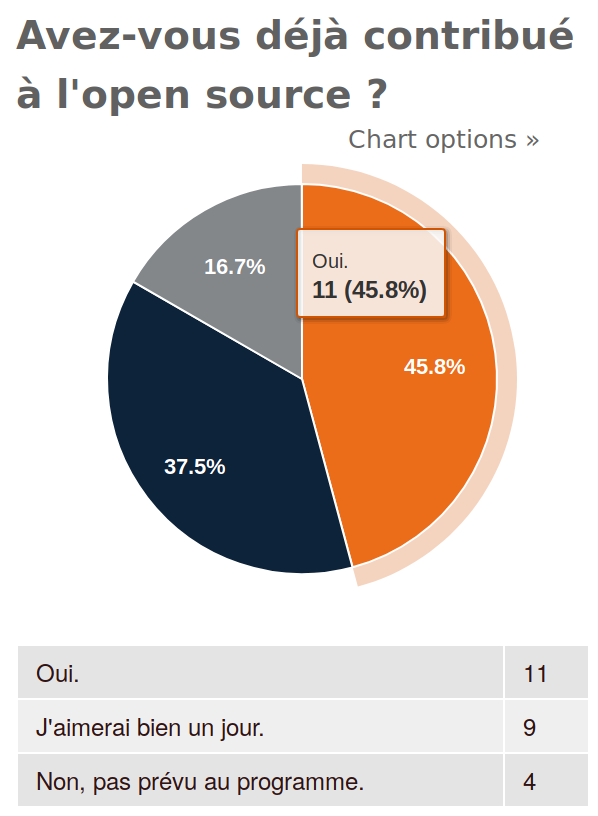
\includegraphics[scale=0.58]{./img/a4}
				\caption{Contribution à l'open source}
			\end{figure}

			L'open source est donc un sujet qui les intéresses et dont \textbf{ils peuvent ou veulent investir du temps en y contribuant}.

			Et ce quelque soit leur domaines d'activité. Sur les 37 personnes qui ont répondu, les domaines d'activités, même si une majoritée est dans l'informatique, sont divers:

			\begin{itemize}[label=\textbullet, font=\LARGE \color{burntorange}]
				\item Edition, Communication, Multimédia
				\item Etude et conseils
				\item Informatique / Télécom
				\item Industriel
				\item Autres
			\end{itemize}

			\begin{figure}[!htb]
				\center
				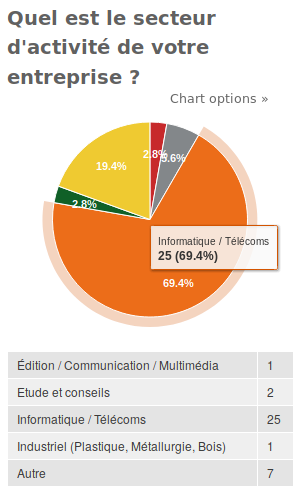
\includegraphics[scale=0.58]{./img/a1}
				\caption{Secteur d'activité des personnes interrogées}
			\end{figure}

			Ainsi \textbf{l'open source n'est pas seulement présent dans l'informatique} et est une préoccupation pour les personnes interrogés.

		\subsection{Le ressenti du consommateur à contribuer}

			J'ai posé une question dans mon questionnaire autour de la perçeption que les gens peuvent avoir dans l'accueil de contribution, s'ils avait des peur ou au contraire qu'il est très agréable de partager avec l'editeur et la communauté ses contributions.\\

			Globalement, aucun frein n'est ressenti à la contribution et son accueil par l'éditeur, même si ces personnes ne contribuent par pour autant:

			\begin{itemize}[label=\textbullet, font=\LARGE \color{burntorange}]
				\item 46\% des interrogés ont répondu que leurs contribution était très bien accueilli, que l'éditeur et la communauté était agréable.
				\item 43\% Ne prennent pas le temps de contribuer mais n'y vois aucun blocage.
				\item Et seulement 11\% ont peur de contribuer et d'être jugé.
			\end{itemize}

			J'en déduis que la moitiée des personnes ont besoin de \textbf{plus de motivations, besoins de contribuer} pour augmenter le nombre de contributions globale.\\

			Dans leur entreprise, ces personnes considèrent pourtant majoritairement que l'open source est essentiel ou nécessaire.\\

			Pour 10 personnes, l'open source est essentiel et ils y attachent beaucoup d'importance.
			12 questionnés disent que l'open source est nécessaire dans leur projets. 8 personnes disent que leur entreprise ne s'en soucie pas vraiment et 5 personnes n'ont jamais entendu parlé d'open source dans leur société.\\

			Je m'aperçoit que \textbf{malgré le degré d'importance considéré de l'open source les personnes interrogés n'en font pas une affaire personnelle}.

			\begin{figure}[!htb]
				\center
				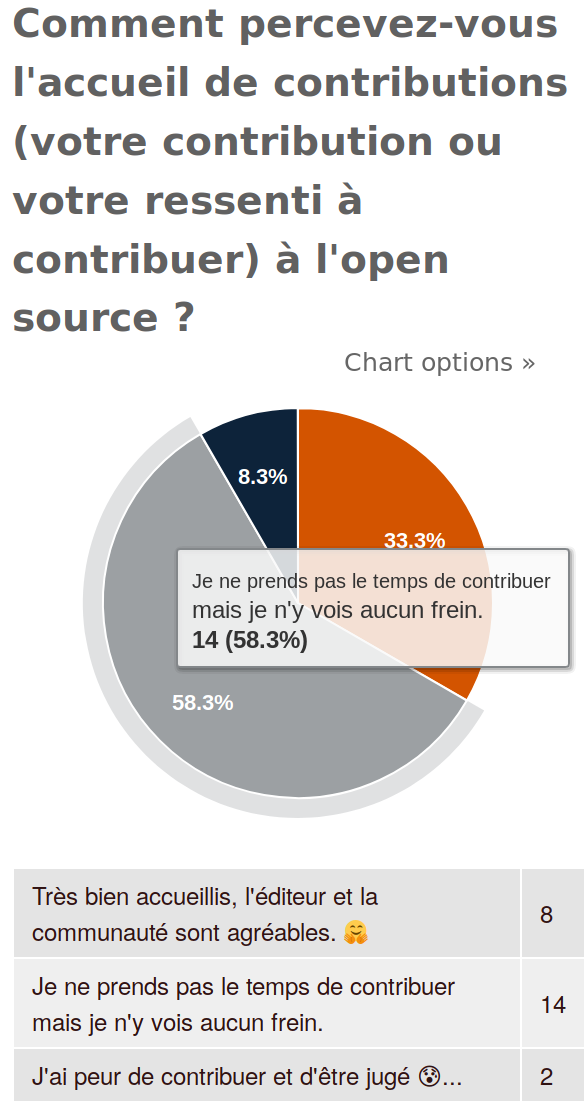
\includegraphics[scale=0.58]{./img/a7}
				\caption{Perception de contribution à l'open source}					
			\end{figure}

			Lors de mon interview avec Florent Garin, il m'informe du manque de contribution présent dans l'open source, et de volonté à contribuer\\

			\begin{center}
				\textit{
				\textquote{
					On ne peux pas sensibiliser une entreprise à participer à un projet open source, l'entreprise va là ou le profit l'appelle.
				}
				}
			\end{center}

			Il explique donc un axe pour inciter les entreprises à contribuer à l'open source:

			\begin{center}
				\textit{
				\textquote{
		 			Il faut plutôt essayer de batir des règles où les entreprises sont incités à contribuer, non pas par acte de bienveillance, mais parce que financièrement et économiquement elles ont des motivations à contribuer.
				}
				}
			\end{center}

			Néanmoins il cloture sa réponse en soulignant que les personnes charitables qui souhaitent contribuer ne doivent pas tant être sensibilisé mais guidés sur la manière de contribuer.\\

			Ainsi il \textbf{reste encore du chemin pour amener les gens à participer et contribuer} activement à l'open source.

		\subsection{Un besoin écouté}

			29 des 37 personnes interrogés ont déclarés qu'après une demande auprès d'un éditeur open source, le besoin du consommateur est suffisemment écouté et ce malgré le fait que les plateformes ne favorisent pas cette communication.

			\begin{figure}[!htb]
				\center
				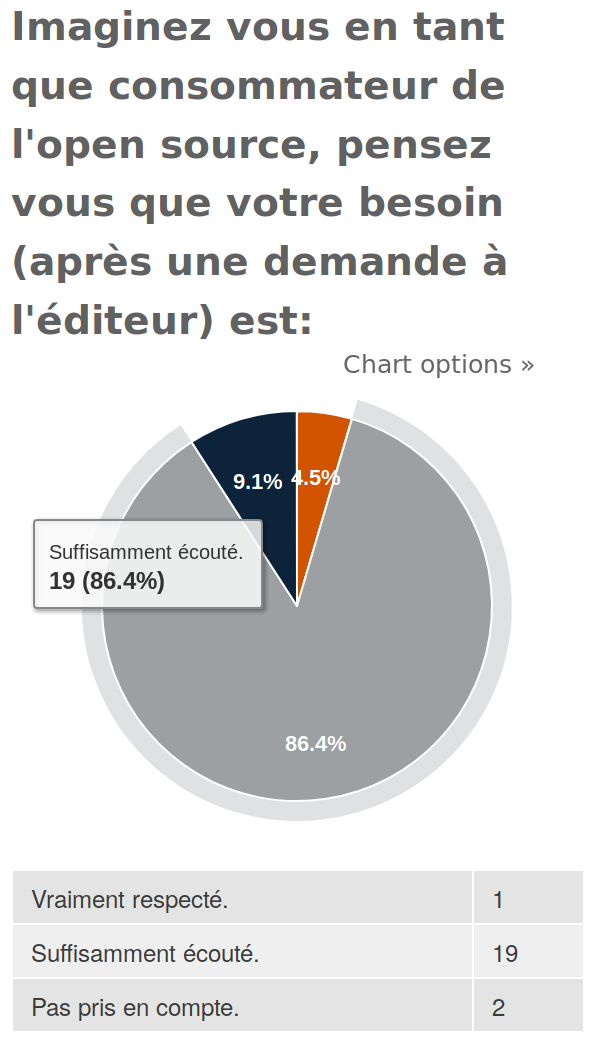
\includegraphics[scale=0.28]{./img/a12}
				\caption{Ecoute du besoin du consommateur}
			\end{figure}

			Ainsi \textbf{la manque de communication dans l'expression du besoin dans l'open source relève d'un problème technique et matériel} plus qu'humain.

			\newpage

			Selon Quentin \bsc{Cazelle}, l'accueil des demandes, remarques à l'éditeur est généralement bien perçu.

			\begin{center}
				\textit{
				\textquote{
		 			Sur les sites comme stackoverflow, github, du moment que les questions sont respectueuses et utiles, les réponses sont constructives et l'on est bien accueillis.
				}
				}
			\end{center}

			Pour Florent \bsc{Garin}, en tant qu'éditeur logiciel open source, le besoin du consommateur est entendu et si plusieurs personnes remontent ce besoin alors on peux supposer qu'il y a un marché derrière qu'il est intéréssant d'y répondre.\\

			Il faut néanmoins garder à l'esprit selon lui qu'il n'y a pas de relation donnant-donnant.

			\begin{center}
				\textit{
				\textquote{
		 			Personne ne doit rien à personne dans cette histoire (l'open source), les éditeurs ne doivent rien aux consommateurs et vice-versa.
				}
				}
			\end{center}


	\section{Marketing de l'open source}

		\subsection{L'école et l'open source}

			\subsubsection{la présence de l'open source}

				Sur une 30aine de personnes qui ont répondu à la question: "Devrait on sensibiliser les gens à l'open source dans les écoles informatiques ?", je constate que 12 de ces personnes ont découvert l'open source par le biais de l'école.

				\begin{figure}[!htb]
					\center
					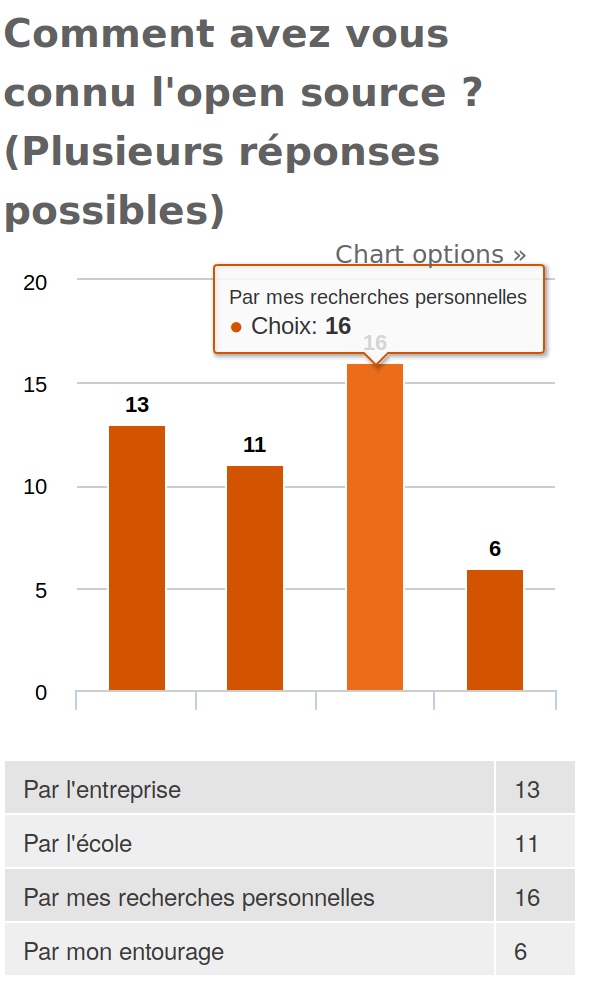
\includegraphics[scale=0.28]{./img/a3}
					\caption{Découverte de l'open source}
				\end{figure}

				A ceci, Quentin \bsc{Cazelle}, qui sort d'une école d'informatique m'indique que son école traitais bien de l'open source et que le sujet était bien présent:

				\begin{center}
					\textit{
					\textquote{
						A l'IUT, j'ai eu des cours sur l'open source, c'était très léger mais on a compris le concept (...) c'est le minimum mais aussi peut-être le maximum que l'on puisse traiter sur ce sujet mais c'est nécessaire. 
					}
					}
				\end{center}

				Rémi \bsc{Buhler}, développeur logiciel, était récemment dans une école informatique et selon lui le sujet n'a pas vraiment été traité.

				\begin{center}
					\textit{
					\textquote{
			 			J'ai entendu parlé de l'open source à l'école dans le cadre de la propriété intellectuelle, mais l'on ne m'a jamais vraiment appris tout ce qui se trouve derrière l'open source et son utilisation à travers le développement logiciel.
					}
					}
				\end{center}

				Egalement, plus de la moitiée des personnes, soit 21 interrogés, ont répondus sur la présence de l'open source à l'école, qu'il était peu ou tout juste assez évoqué.\\

				9 personnes trouvent que les écoles informatiques traitent suffisamment de l'open souce\\

				Seulement 1 personne à déclaré que l'open source était fortement présent dans les écoles informatiques

				\begin{figure}[!htb]
					\center
					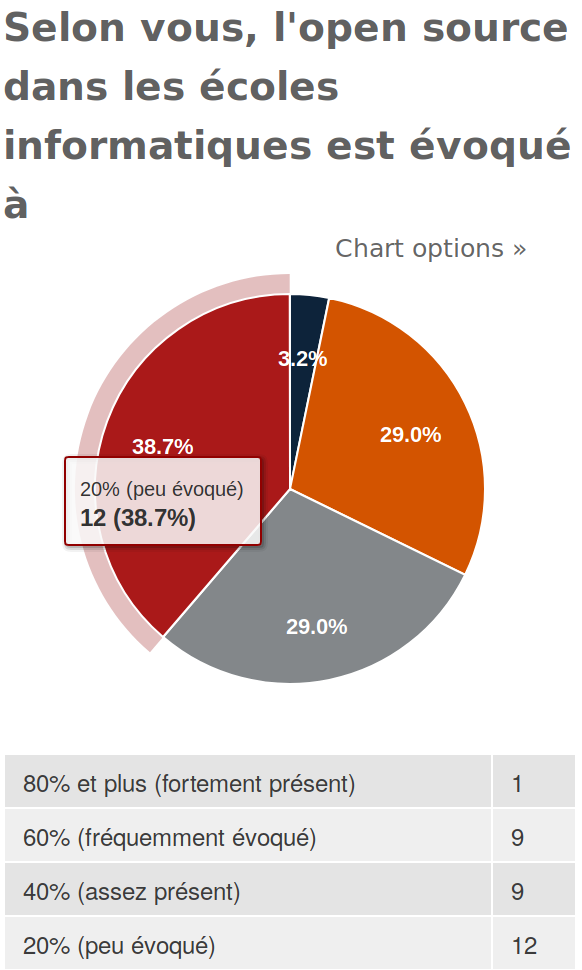
\includegraphics[scale=0.28]{./img/a5}
					\caption{L'open source à l'école}					
				\end{figure}

				Ainsi l'open source n'est pas vraiment présent dans les écoles informatiques et si il l'est, alors il n'est que vaguement évoqué et incomplet.

			\subsubsection{Sensibiliser à l'open source}

				Sur une 30aine de personnes qui ont répondu à la question: "Devrait on sensibiliser les gens à l'open source dans les écoles informatiques ?"\\

				Une majoritée des contributeurs, soit 92\% mentionne que l'on devrait bel et bien sensibiliser les gens à l'open source dans les écoles informatiques\\

				Ceci m'indique que l'enseignement de l'open source dans les école leur à été favorable et qu'ils recommandent donc que le programme contienne un enseignement à l'open source\\

				Seulement 3 personnes, dont 2 qui ont découvert l'open source à l'école, trouvent que c'est déjà fait intrinsèquement au programme.\\

				\begin{figure}[!htb]
					\center
					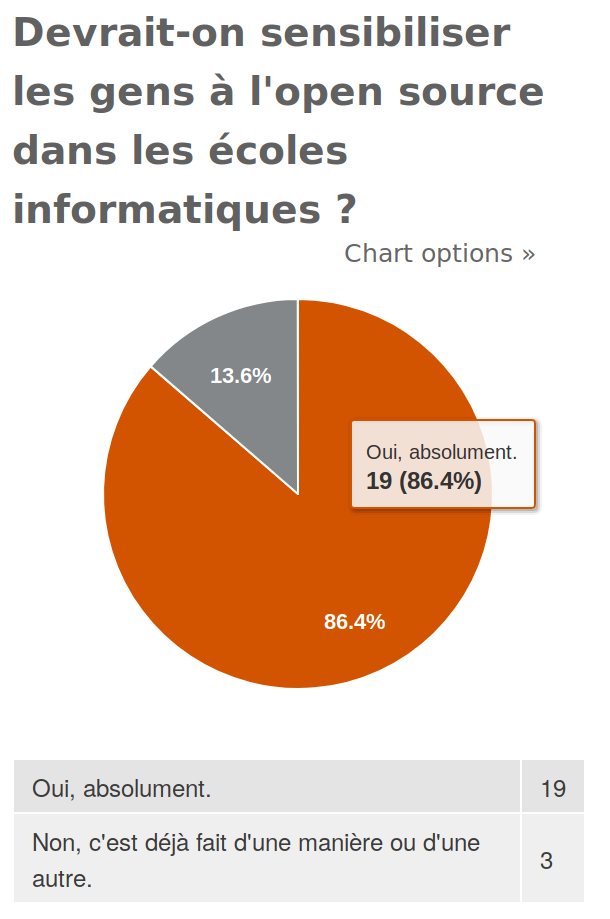
\includegraphics[scale=0.28]{./img/a6}
					\caption{Sensibiliser à l'open source}
				\end{figure}

				\newpage

				Quentin \bsc{Cazelle} me dit que l'open source est une brique nécessaire pour le métier de développeur logiciel et donc les étudiants en informatique.

				\begin{center}
					\textit{
					\textquote{
						Quelqu'un qui fait 5 ans d'étude de développeur et ne sait pas ce qu'est l'open source, c'est une abération!
					}
					}
				\end{center}

				Pour Florent Garin, il n'y a pas véléité à sensibiliser à l'open source les étudiants, mais ils doivent bien connaitre au passage s'ils sont dans une école informatique, ce qu'est l'open source.\\

				J'en conclus que \textbf{ce n'est pas systématique mais l'open source est traité dans les écoles d'informatiques et il se doit de l'être} compte tenu de l'importance qu'il joue dans les entreprises qui accueilleront ces futurs diplomés.

		\subsection{Le support payant}

			Dans l'ensemble des personnes interrogés, une forte majorité indiquent qu'ils ne sont pas contre payer du support pour un logiciel open source. 12 personnes ont répondu qu'il était nécessaire et abordable en général. 22 personnes n'ont pas d'objection à payer pour du support logiciel et comprennent qu'il faille rémunérer l'éditeur d'une certaine façon. Et seulement 3 ont répondu qu'il pensait que l'open source devait être gratuit

			\begin{figure}[!htb]
				\center
				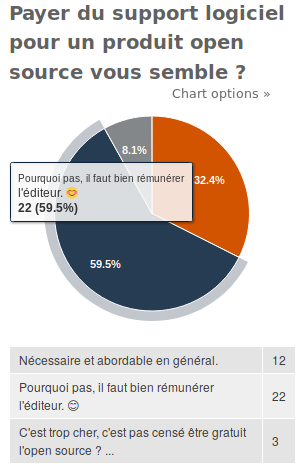
\includegraphics[scale=0.58]{./img/a11}
				\caption{Payer du support logiciel}					
			\end{figure}

			\newpage

			"L'open source attire beaucoup pour sa gratuité" déclare néanmoins Florent \bsc{Garin} et il cible un problème important dans l'abus de ces consommateur qu'ils désigne par le terme de "\gls{leecher}"
			\begin{center}
					\textit{
					\textquote{
						Les consommateurs remontent des anomalies qui ne sont en réalité pas des anomalies mais des demande de support
					}
					}
				\end{center}

			C'est donc que le modèle économique de l'éditeur à travers \textbf{la vente de support logiciel n'est pas un frein à la consommation de l'open source} car beaucoup de personnes interrogées estiment cela comme une moindre chose pour les éditeurs et ne se sentent pas forcément concerné par le coût du support.

		\subsection{Le marketing à faire}

			Florent Garin mentionne que derrière le projet open source il y a finalement un marketing classique qu'il faut faire pour survivre, on espère que le projet open source va suffir en lui même mais ce n'est pas le cas.









